% \documentclass[margin=3mm]{standalone}
% \usepackage{pgfplots}
\pgfplotsset{compat=1.18}

% \begin{document}
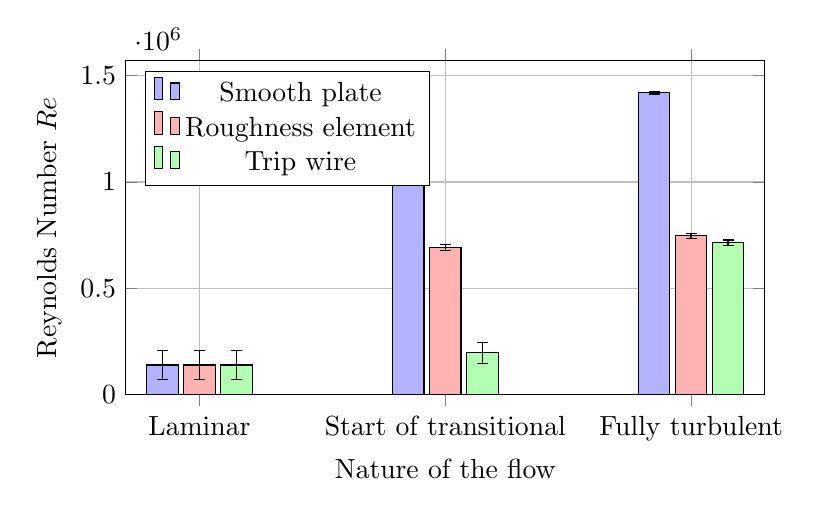
\begin{tikzpicture}
\begin{axis}[
    ybar,
    bar width=0.4cm,           % Adjust width of individual bars
    enlargelimits=0.15,         % Space around the bars
    ylabel={Reynolds Number $Re$},
    xlabel={Nature of the flow},
    symbolic x coords={Laminar, Start of transitional, Fully turbulent},
    xtick=data,
    width=0.8\linewidth,
    height=0.48\linewidth,
    % legend style={at={(0.5,-0.15)}, anchor=north, legend columns=-1},
    legend pos=north west,
    grid=major,
    enlarge y limits={upper=0},
    ymin=0,
]

    % --- 1. Smooth plate ---
    \addplot[
        fill=blue!30,
        error bars/.cd, y dir=both, y explicit,
        error bar style={line width=0.5pt, black}
    ] coordinates {
        (Laminar, 138653.7) +- (0, 69326.8564)
        (Start of transitional, 999846.1) +- (0, 9613.9)
        (Fully turbulent, 1420777.8) +- (0, 6765.6)
    };
    \addlegendentry{Smooth plate}

    % --- 2. Roughness element ---
    \addplot[
        fill=red!30,
        error bars/.cd, y dir=both, y explicit,
        error bar style={line width=0.5pt, black}
    ] coordinates {
        (Laminar, 138653.7) +- (0, 69326.8564)
        (Start of transitional, 693268.6) +- (0, 13865.4)
        (Fully turbulent, 746673.1) +- (0, 12873.7)
    };
    \addlegendentry{Roughness element}

    % --- 3. Trip wire ---
    \addplot[
        fill=green!30,
        error bars/.cd, y dir=both, y explicit,
        error bar style={line width=0.5pt, black}
    ] coordinates {
        (Laminar, 138653.7) +- (0, 69326.8564)
        (Start of transitional, 196086.0) +- (0, 49021.5)
        (Fully turbulent, 713763.7) +- (0, 13467.2)
    };
    \addlegendentry{Trip wire}

\end{axis}
\end{tikzpicture}
% \end{document}